\section{AutoRegressive process}

AutoRegressive models enable us to achieve non-zero auto-covariance ($\gamma(\tau)\neq 0$) using a finite set of coefficients. 
These models are defined as follows:
\[y(t)=a_1y(t-1)+a_2y(t-2)+\cdots+a_m y(t-m)+e(t) \qquad e(t)\sim WN(\mu,\lambda^2)\]
Here, $a_1,a_2,\dots,a_m$ represent the AutoRegressive process coefficients, and $m$ denotes the model order. 
The order of an AutoRegressive model is denoted as AR($m$).

To ensure that an AutoRegressive model is stationary, we consider cases where they represent the steady-state solution of the difference equation.
\begin{example}
    Let's consider the AR($1$) process described by the equation:
    \[y(t)=ay(y-1)+e(t)\qquad e(t) \sim WN(\mu,\lambda^2)\]
    We aim to determine the steady-state solution of this process. 
    It is possible to rewrite the process as:
    \[y(t)=\sum_{i=0}^{+\infty}a^i e(t-1)\]
    This form resembles a Moving Average with an infinite order, with coefficients  $c_0=1,c_1=a,c_2=a^2,\dots,c_i=a^i$. 
\end{example}
Thus, we've discovered that an AutoRegressive model in the steady-state is equivalent to a Moving Average process with infinite order.

\subsection{Operatorial representation}
Let's consider the AR($1$) process described by the equation:
\[y(t)=ay(t-1)+e(t) \qquad e(t)\sim WN(0,\lambda^2)\]
We can employ operatorial representation to derive the transfer function:
\[y(t)\left( 1 -az^{-1} \right)=e(t) \rightarrow y(t)=\dfrac{z}{z-a}e(t)\]
Stability is ensured if the transfer function is asymptotically stable, and the input process is a stochastic stationary process.
By definition,  White Noise is a stationary stochastic process. 
The transfer function is asymptotically stable if $\left\lvert a \right\rvert<1$.
Hence, if $\left\lvert a \right\rvert<1$, $y(t)$ constitutes a stochastic stationary process.
\paragraph*{From AutoRegressive to Moving Average}
Now, let's derive the MA($\infty$) corresponding to the given AutoRegressive model through recursive application of the difference equation or long division. 
The transfer function is:
\[W(z)=\dfrac{1}{1-az^{-1}}=\dfrac{C(z)}{A(z)}\]
To perform long division, we divide $C(z)$ by $A(z)$. 
After an infinite number of steps, we obtain:
\[W(z)=1+az^{-1}+a^2z^{-2}+\dots\]
This result aligns with what we obtained through difference equations, implying that the following condition must hold:
\[\sum_{i=0}^{+\infty} \left\lvert a^2 \right\rvert^i<+\infty \]
However, this condition is automatically satisfied if $\left\lvert a \right\rvert<1$ due to the geometric series.

We have once again demonstrated the relationship between AR($1$) and MA($\infty$) processes. 
However, computing $m_y$ and $\gamma_y(\tau)$ for all $\tau$ using the same tools as those for Moving Average processes is impractical.

\subsection{Mean value}
Let's analyze the AR($1$) process described by the equation:
\[y(t)=ay(t-1)+e(t) \qquad e(t)\sim WN(0,\lambda^2),\left\lvert a \right\rvert<1\]
We aim to compute the mean value, which is constant because the process is stationary:
\[m_y=\mathbb{E}\left[y(t)\right]=\mathbb{E}\left[ay(t-1)+e(t)\right]=a\mathbb{E}\left[y(t-1)\right]+\underbrace{\mathbb{E}\left[e(t)\right]}_0\]
Given that it is a stationary stochastic process, we can state that  $\mathbb{E}\left[\tau\right]=m_y$ for all $\tau$, leading to:
\[m_y=am_y\rightarrow (1-a)m_y=0\rightarrow m_y=0\]

\subsection{Covariance function}
Let's examine the AR($1$) process defined by the function:
\[y(t)=ay(t-1)+e(t) \qquad e(t)\sim WN(0,\lambda^2),\left\lvert a \right\rvert<1\]
We'll begin by computing the covariance function at $\tau=0$, given $m_y=0$:
\begin{align*}
    \gamma_y(0) &=\mathbb{E}\left[ \left(y(t)-m_y\right)\left(y(t)-m_y\right) \right] \\
                &=\mathbb{E}\left[ {\left(y(t)\right)}^2 \right] \\
                &=\mathbb{E}\left[ {\left(ay(t-1)+e(t)\right)}^2 \right] \\      
                &=\mathbb{E}\left[ a^2{y(t-1)}^2+{e(t)}^2+2ay(t-1)e(t) \right] \\     
                &=a^2\underbrace{\mathbb{E}\left[ {y(t-1)}^2\right]}_{\gamma_y(0)} +\underbrace{\mathbb{E}\left[{e(t)}^2\right]}_{\lambda^2} +2a\underbrace{\mathbb{E}\left[y(t-1)e(t)\right]}_{0}  \\    
                &=a^2\gamma_y(0) +\lambda^2 
\end{align*}
Solving $\gamma_y(0)=a^2\gamma_y(0) +\lambda^2$ yields:
\[\gamma_y(0)=\dfrac{\lambda^2}{1-a^2}\]

Next, we'll compute the covariance function at $\tau=1$:
\begin{align*}
    \gamma_y(1) &=\mathbb{E}\left[ \left(y(t)-m_y\right)\left(y(t-1)-m_y\right) \right] \\
                &=\mathbb{E}\left[ \left(ay(t-1)+e(t)\right)y(t-1) \right] \\
                &=\mathbb{E}\left[ a{y(t-1)}^2+e(t)y(t-1) \right] \\     
                &=a\underbrace{\mathbb{E}\left[ {y(t-1)}^2\right]}_{\gamma_y(0)} +\underbrace{\mathbb{E}\left[ e(t)y(t-1) \right]}_0  \\  
                &=a\gamma_y(0) \\
                &=a\dfrac{\lambda^2}{1-a^2}
\end{align*}

Next, we'll compute the covariance function at $\tau=2$:
\begin{align*}
    \gamma_y(2) &=\mathbb{E}\left[ \left(y(t)-m_y\right)\left(y(t-2)-m_y\right) \right] \\
                &=\mathbb{E}\left[ \left(ay(t-1)+e(t)\right)y(t-2) \right] \\
                &=\mathbb{E}\left[ ay(t-1)y(t-2)+e(t)y(t-2) \right] \\     
                &=a\underbrace{\mathbb{E}\left[ y(t-1)y(t-2)\right]}_{\gamma_y(1)} +\underbrace{\mathbb{E}\left[e(t)y(t-2) \right]}_0  \\  
                &=a\gamma_y(1) \\                 
                &=\dfrac{a^2\lambda^2}{1-a^2}
\end{align*}

This pattern continues for $\tau > 1$:
\[\gamma_y(\tau)=a^\tau\dfrac{\lambda^2}{1-a^2}\]
The resulting covariance function for $\tau \geq 0$ is a set of recursive equations, known as the Yule-Walker equations for the AutoRegressive of order one process. 
These equations describe how each covariance depends on the previous one.
\begin{figure}[H]
    \centering
    \begin{subfigure}{0.49\textwidth}
        \centering
        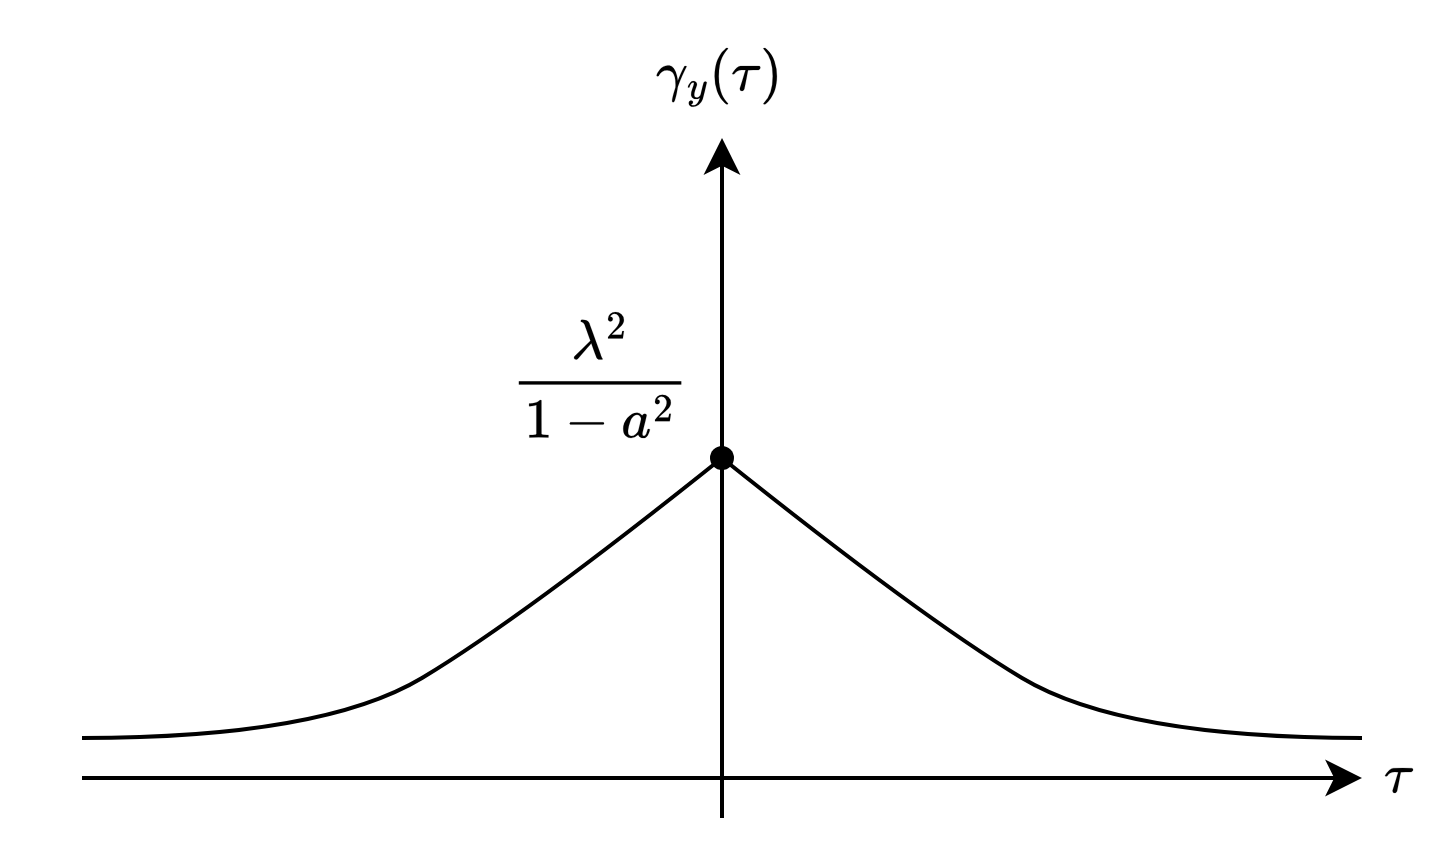
\includegraphics[width=0.85\linewidth]{images/ar1.png} 
        \caption{Parameter $a$ positive}
    \end{subfigure}
    \begin{subfigure}{0.49\textwidth}
        \centering
        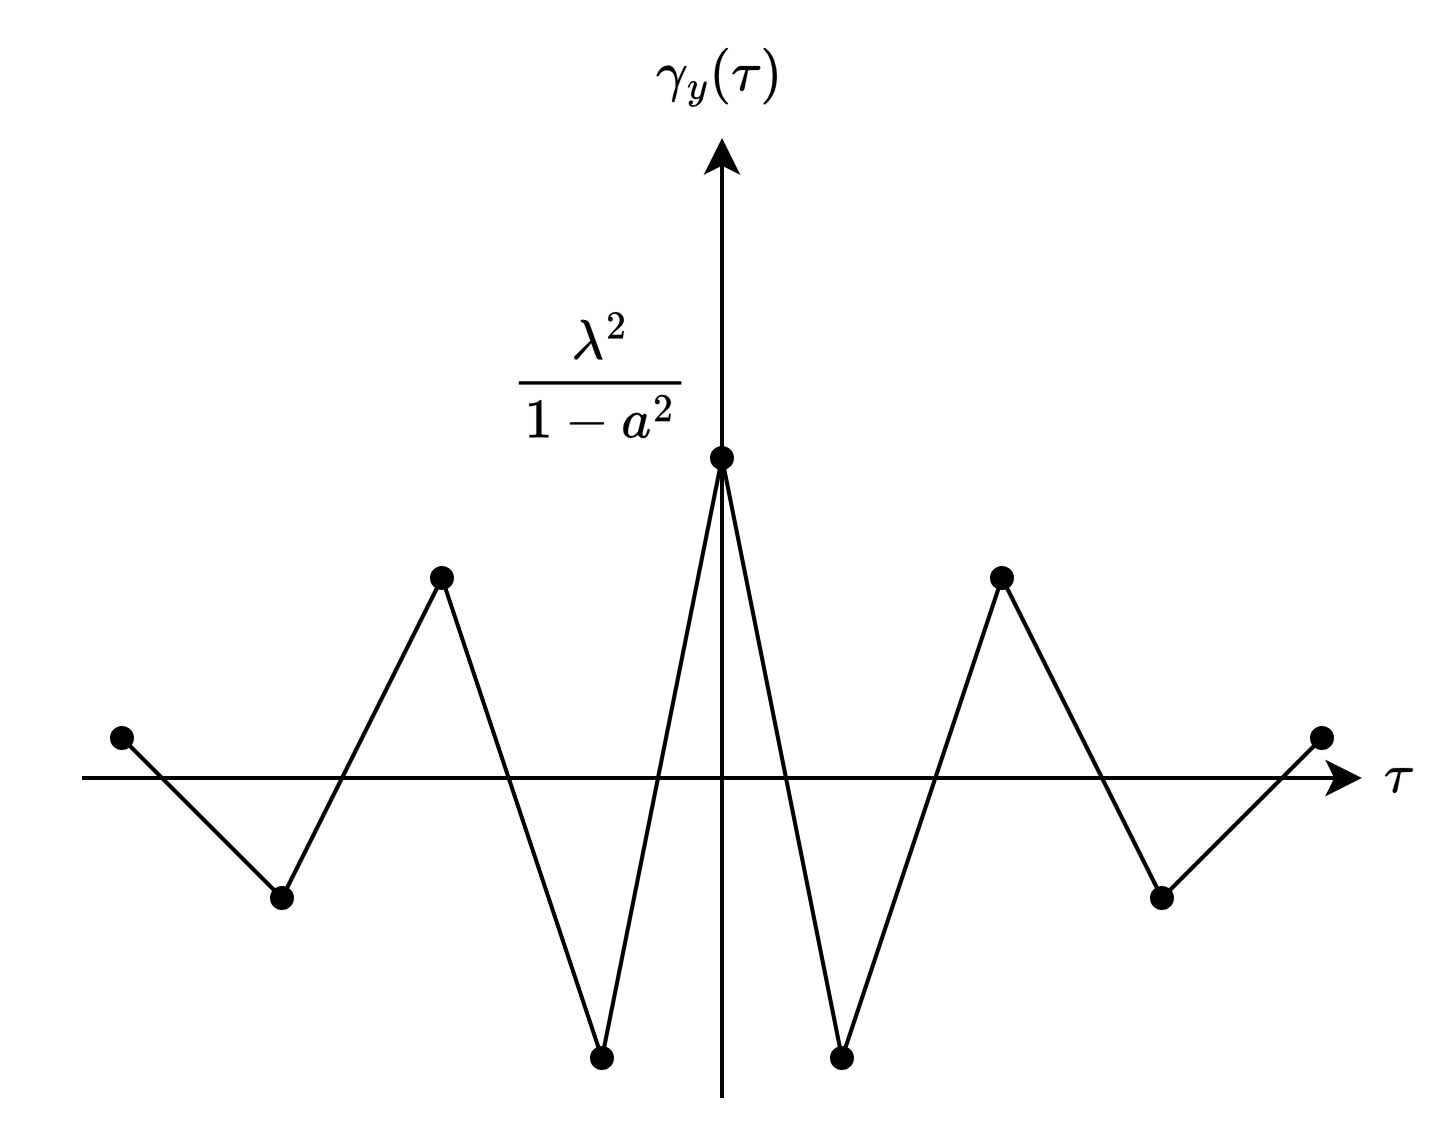
\includegraphics[width=0.75\linewidth]{images/ar2.png}
        \caption{Parameter $a$ negative}
    \end{subfigure}
    \caption{Covariance of a stable AR($1$) process}
\end{figure}

\subsection{White Noise and AutoRegressive covariance}
We have derived the covariance of the AutoRegressive process by computing:
\[\mathbb{E}\left[e(t)y(t-\tau)\right]=0 \qquad \tau >0\]
To demonstrate the validity of this formula, let's begin by examining an MA($\infty$) process, which is equivalent to the AutoRegressive process considered:
\[y(t)=e(t)+ae(t-1)+a^2e(t-2)+\dots\]
Now, let's compute the formula for $\tau = 1$:
\begin{align*}
    \mathbb{E}\left[e(t)y(t-1)\right]   &= \mathbb{E}\left[e(t)\left(e(t-1)+ae(t-2)+a^2e(t-3)+\dots\right)\right] \\ 
                                        &= \mathbb{E}\left[e(t)e(t-1)+ae(t)e(t-2)+a^2e(t)e(t-3)+\dots\right] \\ 
                                        &= \mathbb{E}\left[e(t)e(t-1)\right]+a\mathbb{E}\left[e(t)e(t-2)\right]+a^2\mathbb{E}\left[e(t)e(t-3)\right]+\dots                                      
\end{align*}
Since all expected values involve the  White Noise at different time instants, and since the  White Noise is unpredictable, all these terms become null.
Hence, we have:
\[\mathbb{E}\left[e(t)y(t-1)\right]=0+a\cdot 0+a^2\cdot 0=0\]

Similarly, if we consider the same for any $\tau > 1$, we obtain the same result. 
Therefore, the formula holds true. 
This demonstrates that the covariance expression is valid for the AutoRegressive process.